\chapter{実績}
\section{開発プロセス}
TLVは,OJL(On the Job Learning)の開発テーマとして開発された.OJLとは,
企業で行われているソフトウェア開発プロジェクトを教材とする実践教育であ
り,製品レベルの実システムの開発を通じて創造的な思考力を身につけるとと
もに,単なる例題にとどまらない現実の開発作業を担うことにより,納期,予
算といった実社会の制約を踏まえたソフトウェア開発の実際について学ぶこと
を目的としている.

TLVはプロジェクトベースで開発が行われ、本年度は企業出身者1名と教員1名が
プロジェクトマネージャを務め,筆者含む学生4名が開発実務を行った。進捗の
報告は,週に1度のミーティングと週報の提出により行った.

\subsection{フェーズ分割}
TLVの開発は複数フェーズに分割して行われている。フェーズ1,2,3は主に後藤
ら\cite{goto}によって実施された。本報告書ではフェーズ3以降について述べる。

各フェーズの内容は次に述べる通りである。

\subsubsection{フェーズ1,2,3}
2007年5月~2008年3月までに、一期生によって実施され、TLVの主要機能
の実装が行われた\cite{goto}。

\subsubsection{フェーズ3}
\begin{figure}
\centering
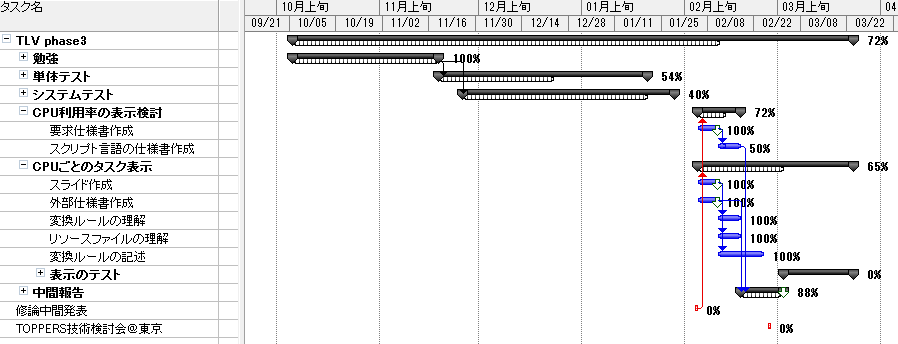
\includegraphics[width=\textwidth]{schedule3.png}
\caption{フェーズ3のスケジュール}\label{fig:sch3}
\end{figure}

\paragraph{期間} 2008年度後期

\paragraph{実施内容}
\begin{itemize}
\item 新規に参加したため、前提となるC\#,TOPPERSの学習を行なった。
\item TLVの各クラスに対する単体テストと、TLV全体に対するシステムテスト
  として、入力ファイルの一部を書き換え不正なファイルを大量に作成し、
  TLVに与えるファジングテスト\cite{fuzzing}を行なった。
\item 次フェーズで行なう予定であった複数のイベントに基づく可視化の要件を検討した。
\end{itemize}

\paragraph{スケジュール}
\figref{fig:sch3}のように、
10月始めから11月中旬にかけて前提となる知識の学習を行ない、
11月中旬から1月末にかけてTLVに対するテストを行ない、
1月末から2月中旬にかけて要件の検討を行なった。

図中の``CPUごとのタスク表示''は、筆者以外の学生が行なった内容である。

\paragraph{成果}
単体テストは328個のメソッドのうち162個のメソッドに対して単体テストを作
成した。システムテストでは不具合を発見できなかった。
機能追加と並行してテストを実施したため、仕様が安定せず効率が悪かった。

また、3月25日にTOPPERS会員に向けに1.0rcをリリースし、要求の収集を行なっ
た。1.0rcのリリースによってユーザインタフェースの改良案,追加の機能要求,
可視化表現項目について要求が得られた.

\subsubsection{フェーズ4}
\begin{figure}
\centering
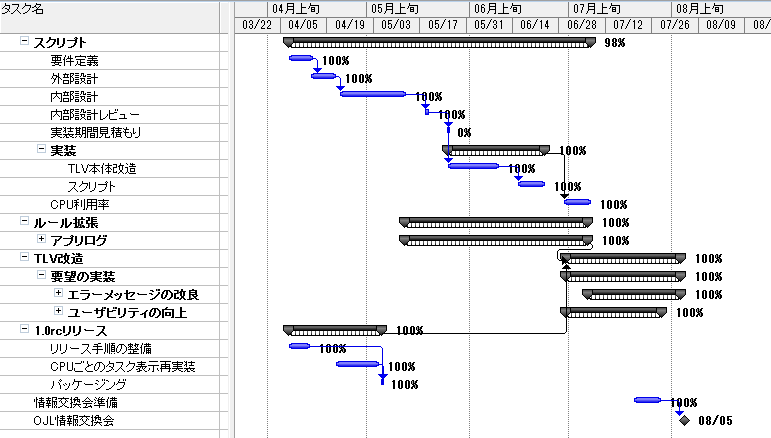
\includegraphics[width=\textwidth]{schedule4.png}
\caption{フェーズ4のスケジュール}\label{fig:sch4}
\end{figure}

\paragraph{期間} 2009年度前期

\paragraph{実施内容}
\begin{itemize}
\item \ref{ch:se}章で述べる複雑な可視化を行なうための機能追加を行なった。
\item 前フェーズで収集した要求のうち、TLVの使いやすさを向上させる要求を実装した。
\end{itemize}

\paragraph{スケジュール} \figref{fig:sch4}のように、
4月始めから7月始めにかけて、
複数のイベントに基づく可視化に対応するためのスクイプト拡張を行なった。
7月始めから8月上旬にかけて、TLVの使いやすさを向上させる要求を実装した。

図中の``アプリログ''は、筆者以外の学生が行なった内容である。

\paragraph{成果}
\ref{ch:se}章で述べる機能を追加した.

5月13日に、TOPPERS会員に対して、
フェーズ3までの内容をまとめた
TLV 1.0をリリースした。

\subsubsection{フェーズ5}
\begin{figure}
\centering
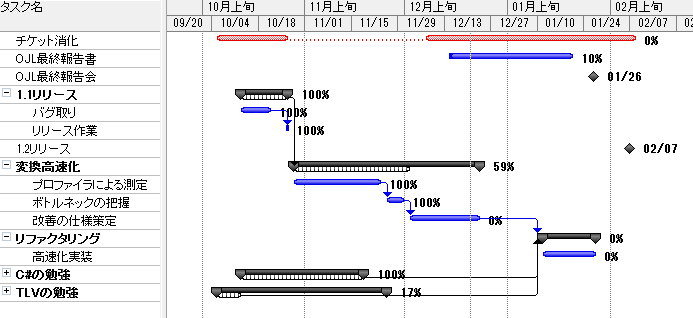
\includegraphics[width=\textwidth]{schedule5.png}
\caption{フェーズ5のスケジュール}\label{fig:sch5}
\end{figure}

\paragraph{期間} 2009年度後期

\paragraph{実施内容}
\begin{itemize}
\item \ref{ch:ref}で述べるように、標準形式トレースログへの変換・図形デー
  タの生成に関するソースコードの調査、およびリファクタリング方針の決定
  を行なった。
\item 新たに三期生が参加したため、課題を与えるなどの指導を行なった。
\end{itemize}

\paragraph{スケジュール} \figref{fig:sch5}のように、10月始めから11月末にかけて、
TLVの解析を行なった。12月始めから12月末にかけてリファクタリング案の策定
を行なった。

\paragraph{成果物}
\ref{ch:ref}章で述べるリファクタリング方針を決定した。また、TOPPERS会員
に対してRC版をリリースし、その後一般向けにTLV1.1をリリースした。

\begin{itemize}
\item 10月1日にTOPPERS会員に対してTLV 1.1rc1を公開。
\item rc1の不具合を修正し、10月26日にTOPPERS会員に対してTLV 1.1rc2を公開。
\item 11月9日に一般向けにTLV 1.1を公開。
\end{itemize}

\section{チケット終了率}
\begin{figure}
\centering
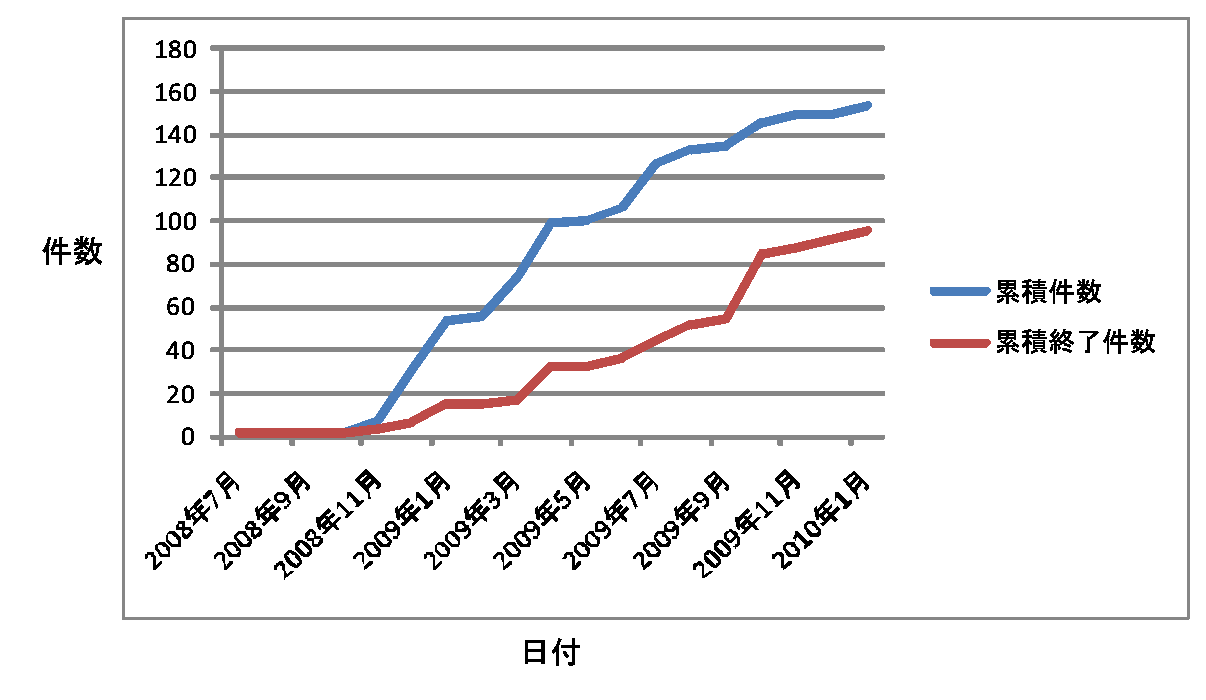
\includegraphics[width=\textwidth]{ticket.eps}
\caption{チケット累積件数}\label{ticket}
\end{figure}

今期のOJLで収集した要求・不具合はすべてTracのチケットとして管理した。
フェーズ3で新た
に追加されたチケット件数は20件、終了したチケットは2件、フェーズ4で新た
に追加されたチケット件数は52件、終了したチケットは27件、フェーズ5で新た
に追加されたチケット件数は27件、終了したチケットは51件であった。

チケットの累積件数・累積終了件数を\figref{ticket}に示す。図より、
一般的な要求曲線を描いていることがわかる。



\section{発表実績}
平成21年度 情報処理学会 第139回 システムLSI設計技術(SLDM)研究会において
発表\cite{ipsj}を行ない、情報処理学会山下記念研究賞/学生奨励賞を受賞した。

Embedded Technology 2009(ET2009)
\footnote{\URL{http://www.jasa.or.jp/et/}}
において、ブース出展及びTLVの一般公開に
ついてプレス発表を行なった。

\section{活用事例}
名古屋大学大学院情報科学研究科付属組込みシステム研究センター(NCES)
\footnote{\URL{http://www.nces.is.nagoya-u.ac.jp/}}内の
7件のプロジェクトのうち、2件のプロジェクトによって利用されている。
また、同NCESのコンソーシアム型共同研究によっても利用されている。
